\chapter{Theoretical and Experimental Overview} \label{ch::theory_exp}
\ifpdf
\graphicspath{{Chapters/Theory/Figs/Raster/}{Chapters/Theory/Figs/PDF/}{Chapters/Theory/Figs/}}
\else \graphicspath{{Chapters/Theory/Figs/Vector/}{Chapters/Theory/Figs/}}
\fi

\section{Deep Inelastic Scattering}
To understand the structure of the nucleon it is useful to first introduce the
original process which described the nucleon as having a sub-structure.  This
process is the Deep Inelastic Scattering (DIS) process where a lepton impinges
on a nucleon denoted as

\begin{equation}
l(\ell) + N(P) \rightarrow l(\ell') + X(P_X),
\end{equation}
\noindent
where $l$ denotes a lepton, $N$ denotes a nucleon, $X$ represents all products
not detected and $\ell$, $\ell'$, $P$ and $P_X$ are the four momentum for their
respective lepton or nucleon.  This process is an electromagnetic reaction where
a the lepton is scattered via virtual photon exchange with the nucleon.  The
leading order Feynman diagram for this reaction is shown in
Fig.~\ref{fig::DIS_LO}.

\begin{figure}[h!t]
  \centering
  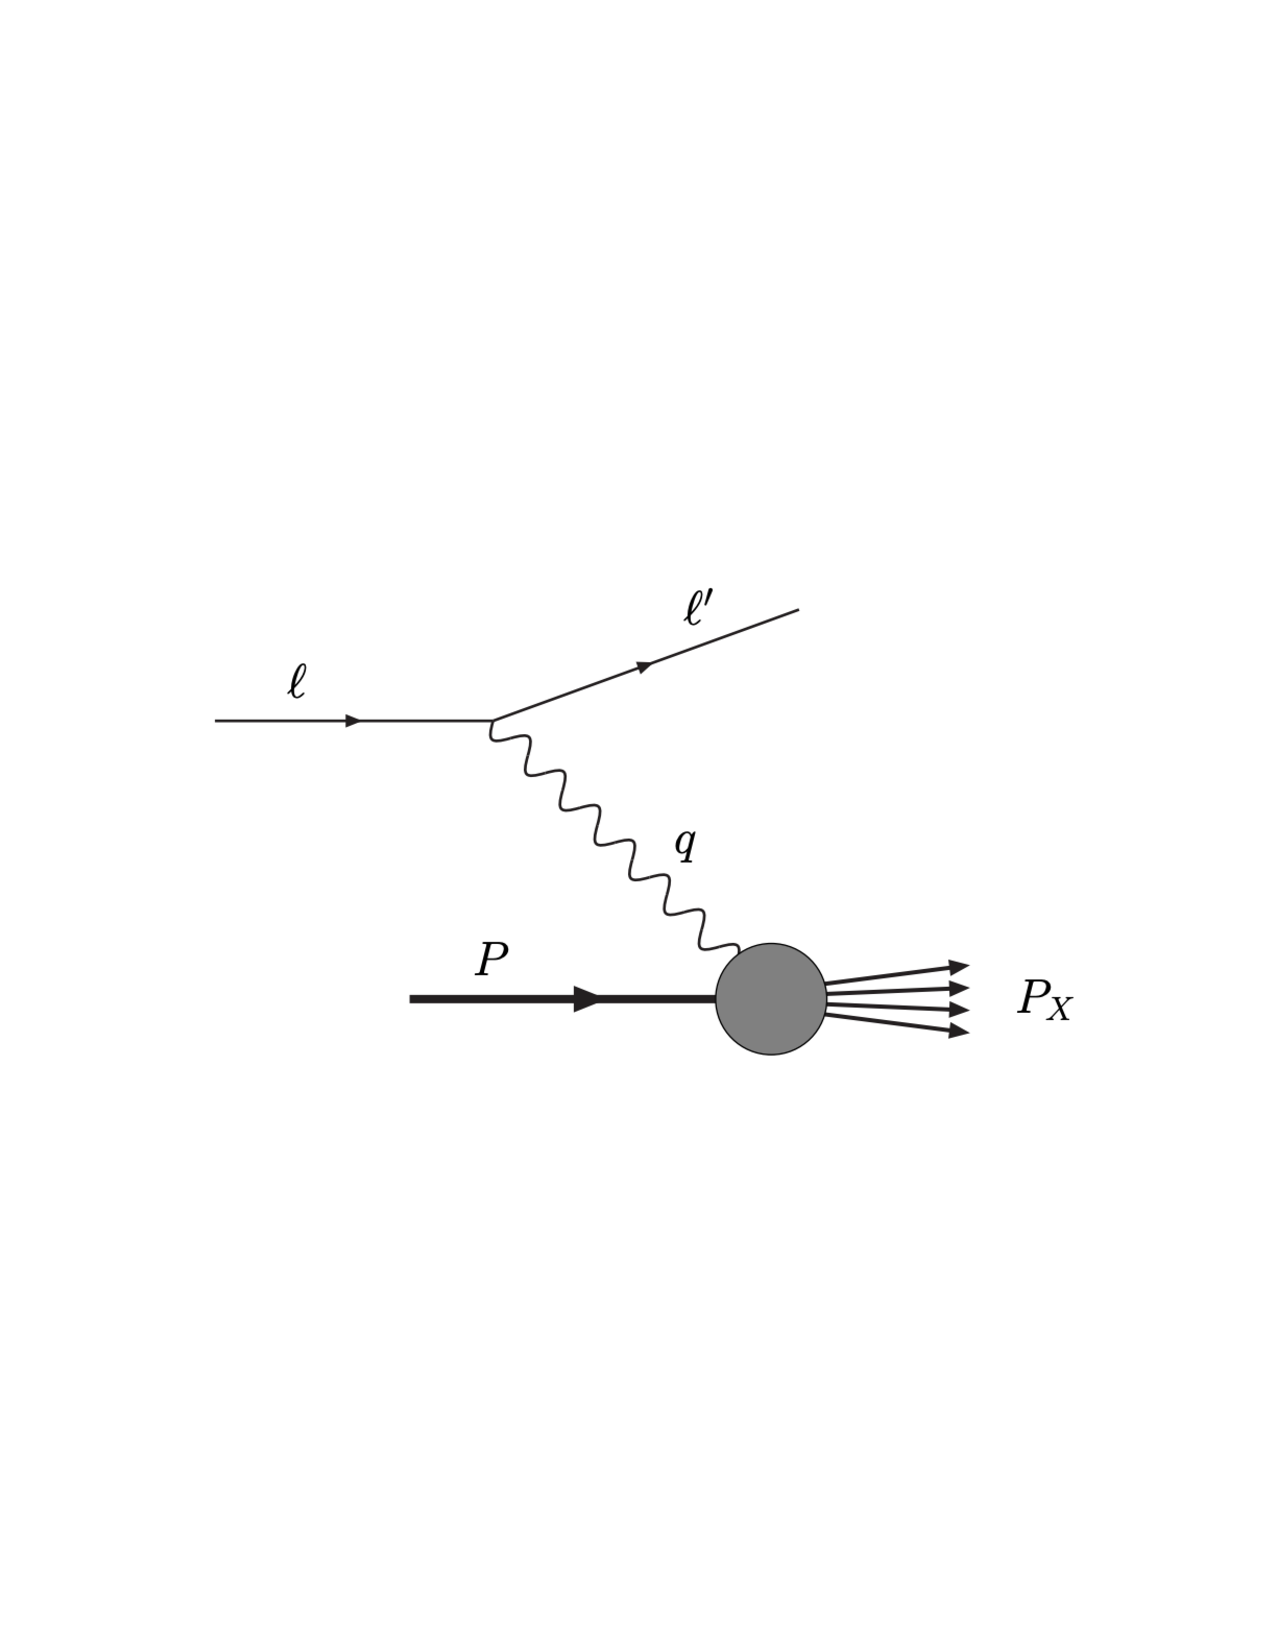
\includegraphics[width=0.5\textwidth, trim=3cm 9cm 3cm 9cm, clip]{DIS_LO}
  \caption{The leading order Feynman diagram for deep inelastic scattering}
  \label{fig::DIS_LO}
\end{figure}

DIS is traditionally studied with a high energy lepton beam and a fixed nuclear
target.  The initial state kinematics are described by

\begin{equation}
  s = (\ell+P)^2 \quad \mathrm{or} \quad E,
\end{equation}
\noindent
where $s$ is the center of mass energy and $E$ is the energy of the lepton beam.
The detected reaction kinematics in the lab frame are described by

\begin{multicols}{2}
  \noindent
  \begin{equation}
    \label{equ::DIS_Q2}
    Q^2 = -q^2 = -(\ell - \ell')^2 \approx EE'(1-\cos\theta )
  \end{equation}
  \begin{equation}
      \label{equ::BjorkenX}
      x = \frac{Q^2}{2P \cdot q} = \frac{Q^2}{2M\nu}
  \end{equation}
\end{multicols}

\begin{multicols}{2}
  \noindent
  \begin{equation}
    \nu = E - E'
  \end{equation} 
  \begin{equation}
    \label{equ::inelasticity}
    y = \frac{P \cdot q}{P \cdot \ell} = \frac{E - E'}{E} = \frac{\nu}{E}
  \end{equation} 
\end{multicols}

\begin{multicols}{2}
  \noindent
  \begin{equation}
    \label{equ::DIS_W}
    W^2 = (P+q)^2
  \end{equation}
\end{multicols}

\noindent
where $q$ is the virtual photon four momentum, $E'$ is the scattered leptons
energy, $x$ is Bjorken x, $\nu$ is the change in energy of the scattered lepton,
$y$ is the inelasticity and $W^2$ is invariant mass of hadron final state.  In
the last relation from Eq.~\ref{equ::DIS_Q2}, $\theta$ is the scattering angle
of the lepton with respect to the beam and the approximation is only true when
the lepton mass is assumed to be zero.  In Eq.~\ref{equ::BjorkenX}, $M$ is the
nucleon mass.  In the parton model, section~\ref{sec::parton_model}, $x$ has the
interpretation as being the momentum fraction of the struck parton with respect
to its parent hadron and therefore $x$ ranges between 0 and 1.  The
inelasticity, $y$, measure the proportional lepton energy reduction and
therefore takes on a value between 0 and 1.

The process is called deep if $Q^2 >> M^2$ and inelastic if $y < 1$.  For
practical purposes in experiments, the deep inelastic criteria corresponds to a
$Q^2 > 1~GeV$ and $W^2 > M^2$.  As can be seen in
Eq.~[\ref{equ::DIS_Q2}-\ref{equ::DIS_W}], not all the variables are independent.
DIS is described by two independent variables usually given by ($x$, $Q^2$) or
($x$, $y$).  For reference, in the limit as $y \to \; 1$ the process becomes
elastic scattering and can then be described by only one independent variable.

The cross-section for DIS is defined as~\cite{Barone:2001sp}
\begin{equation}
  \label{equ::DIS_xsection}
  \mathrm{d}\sigma =
  \frac{1}{4P\cdot \ell}\frac{e^4}{Q^4} L_{\mu\nu}W^{\mu\nu}
  2\pi\frac{\mathrm{d}^3\ell'}{(2\pi)^32E'}
\end{equation}
\noindent
where $L_{\mu\nu}$ is the leptonic tensor and $W^{\mu\nu}$ is the hadronic
tensor.  The leptonic tensor describes free leptons and can therefore be
calculated in perturbation theory.  It can be decomposed into a systematic
spin-independent tensor and an anti-symmetric spin-dependent tensor.  Summing
over all the possible spins of the lepton beam, the leptonic tensor is

\begin{equation}
  L_{\mu\nu} = 2\Big(\ell_{\mu}\ell'_{\nu} + \ell_{\nu}\ell'_{\mu} -
  g_{\mu\nu}\ell \cdot \ell' \Big) +
  2m\epsilon_{\mu\nu\rho\sigma}s^{\rho}q^{\sigma}
\end{equation}
\noindent
where $m$ is the lepton mass and $s^{\rho}$ is the spin four vector of the
lepton.

Generically the hadronic tensor is defined as
\begin{equation}
  W^{\mu\nu} = \frac{1}{2\pi}
  \int \mathrm{d}^4\xi e^{iq \cdot \xi}
  \langle PS | J^{\mu}(\xi)J^{\nu}(0) | PS \rangle
\end{equation}
\noindent
where $J$ is an electromagnetic current and $|PS \rangle$ represents the nucleon
with momentum $P$ and spin $S$.  The hadronic tensor describes a hadron bound
together by quantum chromo-dynamics (QCD).  As of yet there is no known
technique for calculating the hadronic tensor in a perturbation theory or
otherwise.  Instead the hadronic tensor can be written in the most general
Lorentz invariant form using structure functions to parameterize the
non-perturbative nature of the tensor.  With the use of these structure
functions, the differential DIS cross-section can be written
\begin{equation}
  \label{equ::DIS_diffxsection}
  \frac{\mathrm{d}\sigma}{\mathrm{d}x\mathrm{d}y} =
  \frac{8\pi\alpha^2ME}{Q^4}
  \Big\{
  xy^2F_1(x, Q^2) + \Big(1-y\Big)\frac{F_2(x, Q^2)}{x}
  + c_1(y, \frac{Q^2}{\nu}) g_1(x, Q^2) + c_2(y, \frac{Q^2}{\nu}) g_2(x, Q^2)
  \Big \}
\end{equation}
\noindent
where $\alpha$ is the electromagnetic coupling constant; $F_1$, $F_2$, $g_1$,
$g_2$ are structure functions; and $c_1$ and $c_2$ are functions which depend on
the polarization of the target.  The SLAC collaboration measured the structure
functions, $F_1$ and $F_2$, and found mild variations as a function
$Q^2$~\cite{Bloom:1969kc,Breidenbach:1969kd}.  This phenomenon now known as
Bjorken scaling lead to the theory of the parton model~\cite{Bjorken:1969ja}.
Fig.~\ref{fig::F2} shows the $F_2$ structure function which is approximately
constant as a function of $Q^2$.

\begin{figure}[h!t]
  \centering
  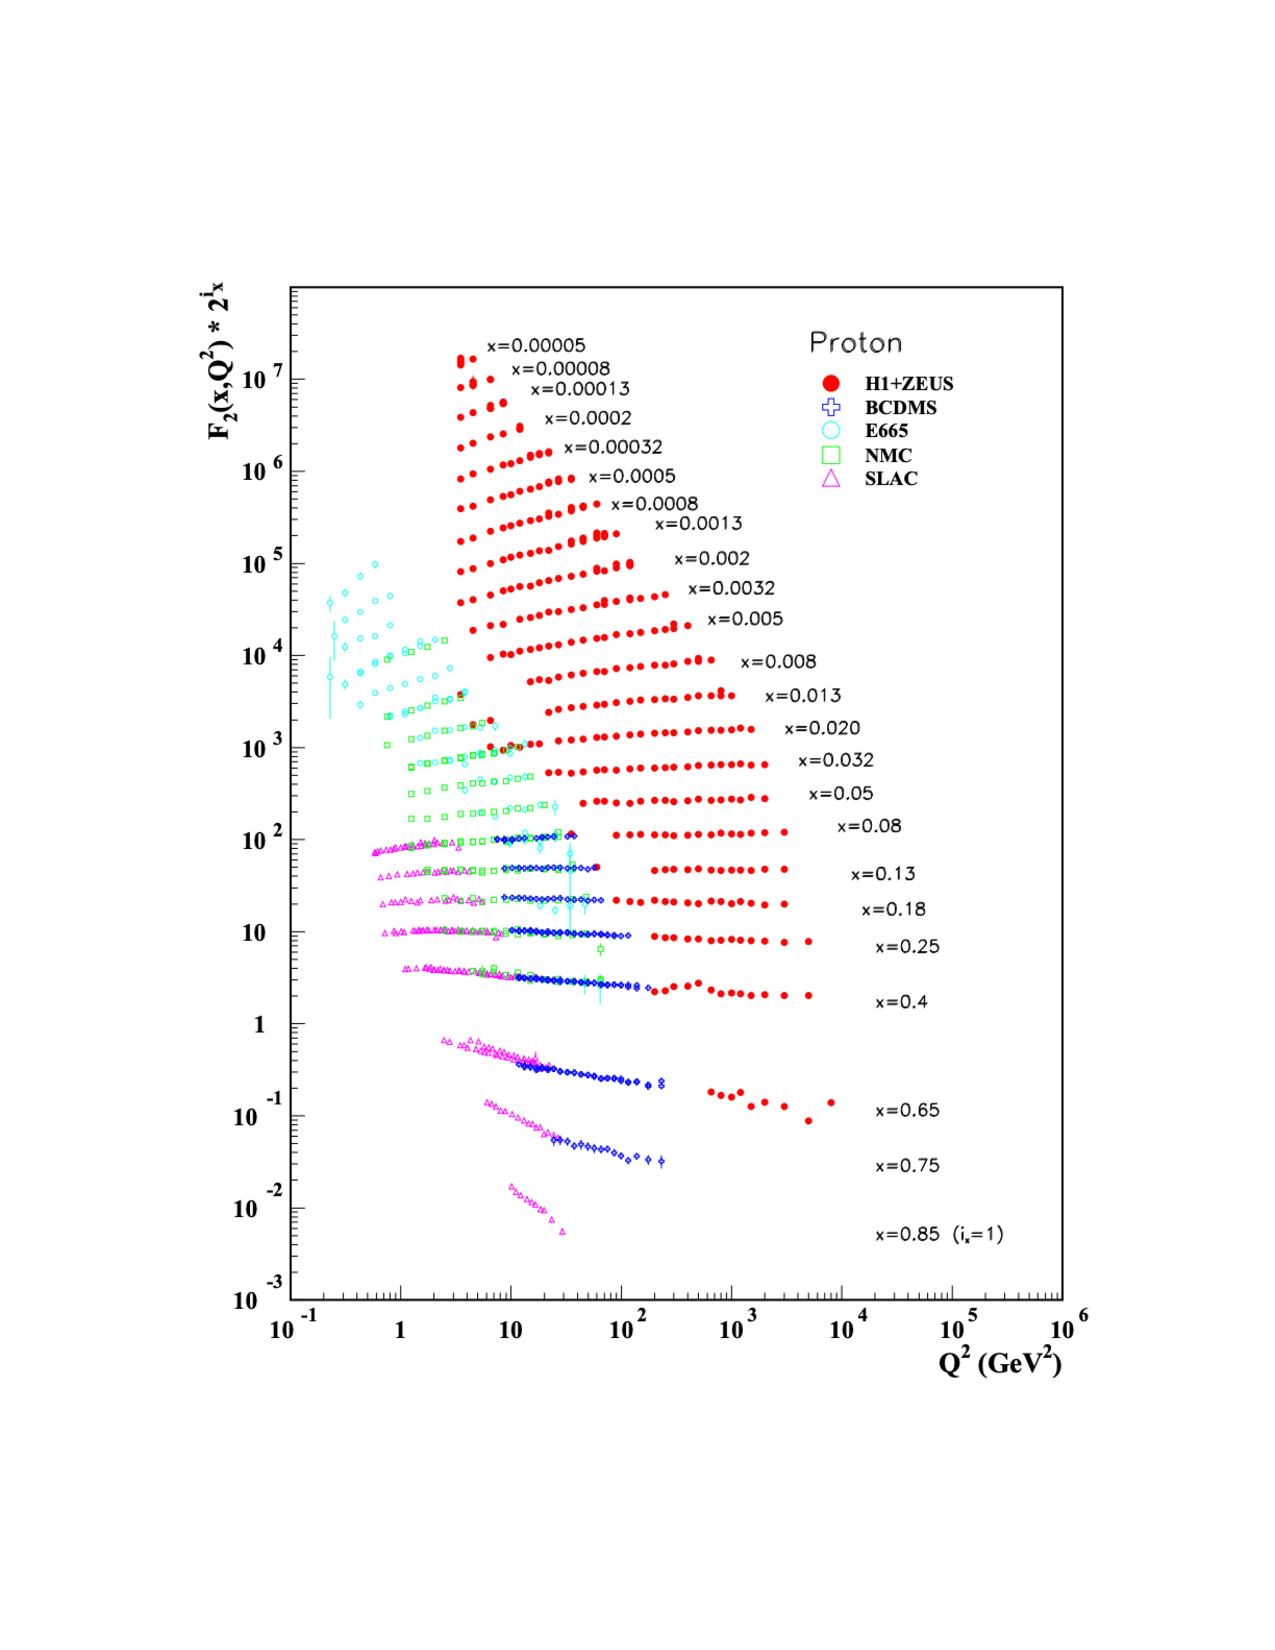
\includegraphics[width=0.5\textwidth, trim=3cm 4cm 3cm 4cm, clip]{F2}
  \caption{The $F_2$ structure function measured by several experiments.  Note
    that the data is shifted up by a factor $2^{i_x}$ to see the $x$ dependence.
    Image taken from~\cite{Tanabashi:2018oca}}
  \label{fig::F2}
\end{figure}


\section{The Parton Model} \label{sec::parton_model}
The parton model is described in what is called an infinite momentum frame where
the nucleon is moving which large momentum.  In the parton model the nucleon, in
high energy scattering processes, is considered to be composed of point like
constituent mass-less particles called partons.  At high energy scattering the
QCD strong force binding the partons becomes asymptotic small and therefore the
partons appear to be free.  The cross-section in DIS can then be described as a
lepton scattering incoherently off a free parton in the nucleon.  In the parton
model the hadron tensor for scattering off a quark can be written
as~\cite{Barone:2001sp}

\begin{dmath}
  W^{\mu\nu} = \frac{1}{2\pi} \sum_q e_q^2 \sum_X
  \int \frac{\mathrm{d}^3 P_X}{(2\pi)^32E_X}
  \int \frac{\mathrm{d}^4k}{(2\pi)^4}
  \int \frac{\mathrm{d}^4k'}{(2\pi)^4} \delta(k^{\prime2}) \times
       [\bar{u}(k')\gamma^{\mu}\langle X | u(k) | PS \rangle]*
       [\bar{u}(k')\gamma^{\nu}\langle X | u(k) | PS \rangle]
       \times (2\pi)^4\delta^4(P-k-P_X)(2\pi)^4\delta^4(k+q-k'),
\end{dmath}
\noindent
where $e_q$ is the electric charge of quark flavor $q$; and $u$ and $\bar{u}$
are free Dirac spinors.  This hadronic tensor can be simplified by introducing
the quark-quark correlation matrix as

\begin{equation}
  \Theta_{ij}(k, P, S) =
  \sum_X \int \frac{\mathrm{d}^3 P_X}{(2\pi)^32E_X}(2\pi)^4\delta^4(P-k-P_X)
  \times \langle PS | \phi_j(0) | X \rangle \langle X | \phi_i(0) | PS \rangle,
\end{equation}
\noindent
where $\phi(\xi) = e^{-ip \cdot \xi}u(p)$ is a quark field.  Using the
quark-quark correlation matrix, the hadronic tensor can be written as

\begin{equation}
  W^{\mu\nu} = \sum_q e_q^2 \int \frac{\mathrm{d}^4k}{(2\pi)^4}
  \int \frac{\mathrm{d}^4k'}{(2\pi)^4} \delta(k^{\prime2})
  (2\pi)^4\delta^4(k+q-k')\times \mathrm{Tr}
  [ \Theta \gamma^{\mu}\slashed{k'}\gamma^{\nu} ].
\end{equation}
\noindent
In the cases of unpolarized or longitudinally polarized DIS the lead order
contributing terms from the quark-quark correlator
are~\cite{Mulders:1995dh,Boer:1997nt,Bacchetta:2006tn}

\begin{equation}
  \label{equ::simpleQQcorr}
  \Theta = \frac{1}{2}
  \Big(
  f_1(x)\slashed{P} +
  g_{1L}(x)\lambda\gamma_5\slashed{P}
  \Big)
\end{equation}
\noindent
where $\lambda$ is the longitudinal polarization of the hadron.  The hadronic
tensor simplifies to a symmetric contribution and an anti-symmetric
contribution~\cite{Barone:2001sp}

\begin{equation}
  \label{equ::simpleHadronTensor}
  W^{\mathrm{symmetric}}_{\mu\nu} = \frac{1}{P\cdot q} \sum_q e_q^2
  \Big( (k_{\mu}+q_{\mu})P_{\nu} + (k_{\nu}+q_{\nu})P_{\mu}-g_{\mu\nu}
  \Big) f_1^q(x),
\end{equation}
\begin{equation}
  W^{\mathrm{anti-symmetric}}_{\mu\nu} =
  \lambda\epsilon_{\mu\nu\rho\sigma}(k_{\nu}+q_{\nu})P^{\rho}\sum_q e^2_q
  g^q_{1L}(x),
\end{equation}
\noindent
where in Eq.~\ref{equ::simpleQQcorr} $f_1$ and $g_1$ are two parton distribution
functions (PDFs).  $f_1$ is interpreted as the quark number density and $g_{1L}$
is interpreted as the total quark helicity distribution in a hadron.  $f_1$ is
then refers to the density of unpolarized quarks in a hadron and $g_{1L}$ refers
to the density of quarks longitudinally polarized in the same longitudinal
direction as the hadron.  To make this explicit, $f_1$ and $g_{1L}$ can be
written

\begin{multicols}{2}
  \noindent
  \begin{equation}
    f_1 = f_1^{+} + f_1^{-},
  \end{equation}
  \begin{equation}
    g_{1L} = f_1^{+} - f_1^{-},
  \end{equation}
\end{multicols}
\noindent
where + and - denote the helicity.  To be clear the parton distribution $g_{1L}$
is not the same as the structure function $g_1$.

The unpolarized quark number density, $f_1$, has been extracted from global
analysis of several experiments~\cite{Rojo_2015}.  Fig.~\ref{fig::NNPDF_10GeV}
shows the current $xf_1$ values and confidence intervals for different quarks
and gluons specifically in the proton.

\begin{figure}[h!t]
  \centering 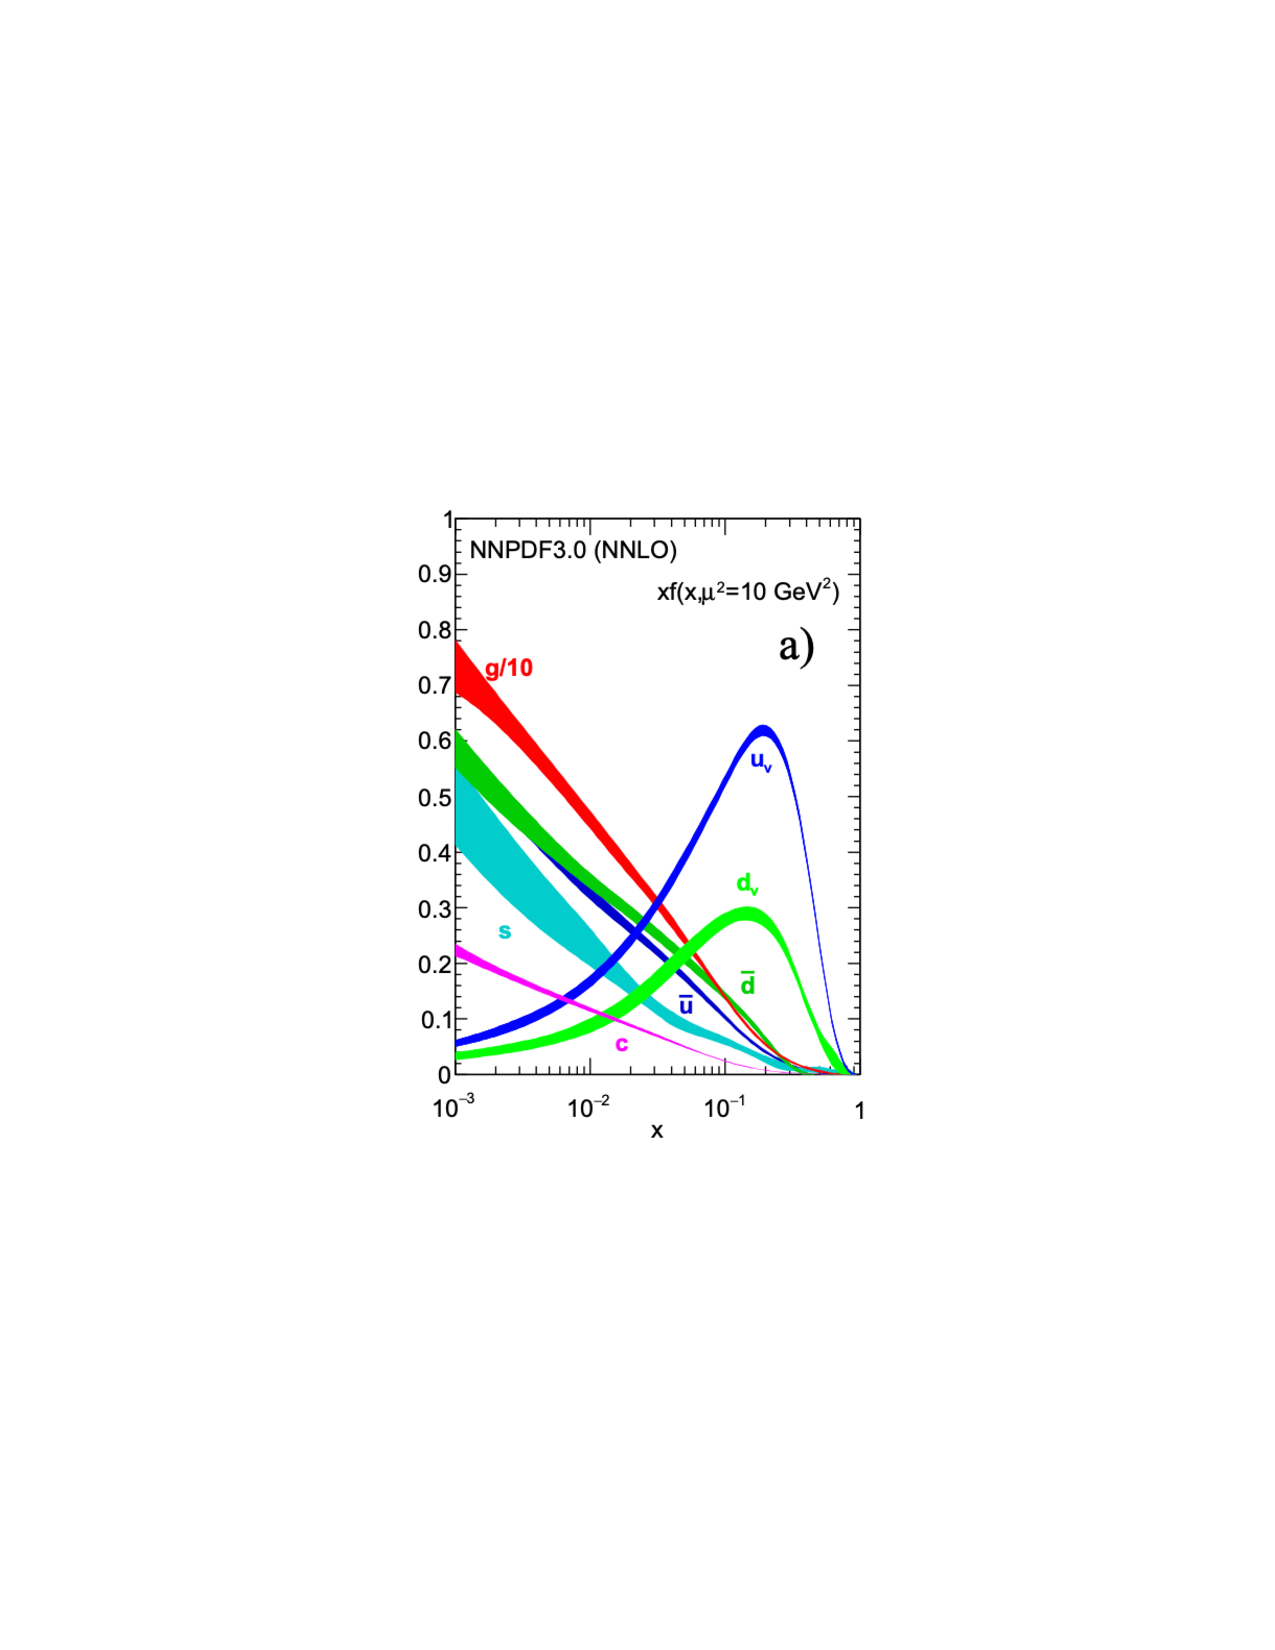
\includegraphics[width=0.5\textwidth,trim=6cm 9cm 6cm 8cm,
    clip]{NNPDF_10GeV}
  \caption{The unpolarized parton distribution functions times the momentum
    fraction.  The different color correspond to different quarks or gluons.
    Image taken from~\cite{Tanabashi:2018oca}}
  \label{fig::NNPDF_10GeV}
\end{figure}

The longitudinal spin structure, $g_{1L}$ has also been measured at SMC, HERMES,
and COMPASS~\cite{Adeva:1997is,PhysRevLett.92.012005,Savin:2011zz}.  The global
analysis fit is shown in Fig.~\ref{fig::Proton_g1L} using the parameterizations
from NNPDF2014, AAC2008, DSSV2008 and
LSS2010~\cite{Harland-Lang:2016yfn,Abt:2016vjh,Nocera:2014gqa,Hirai:2008aj}.

\begin{figure}[h!t]
  \centering 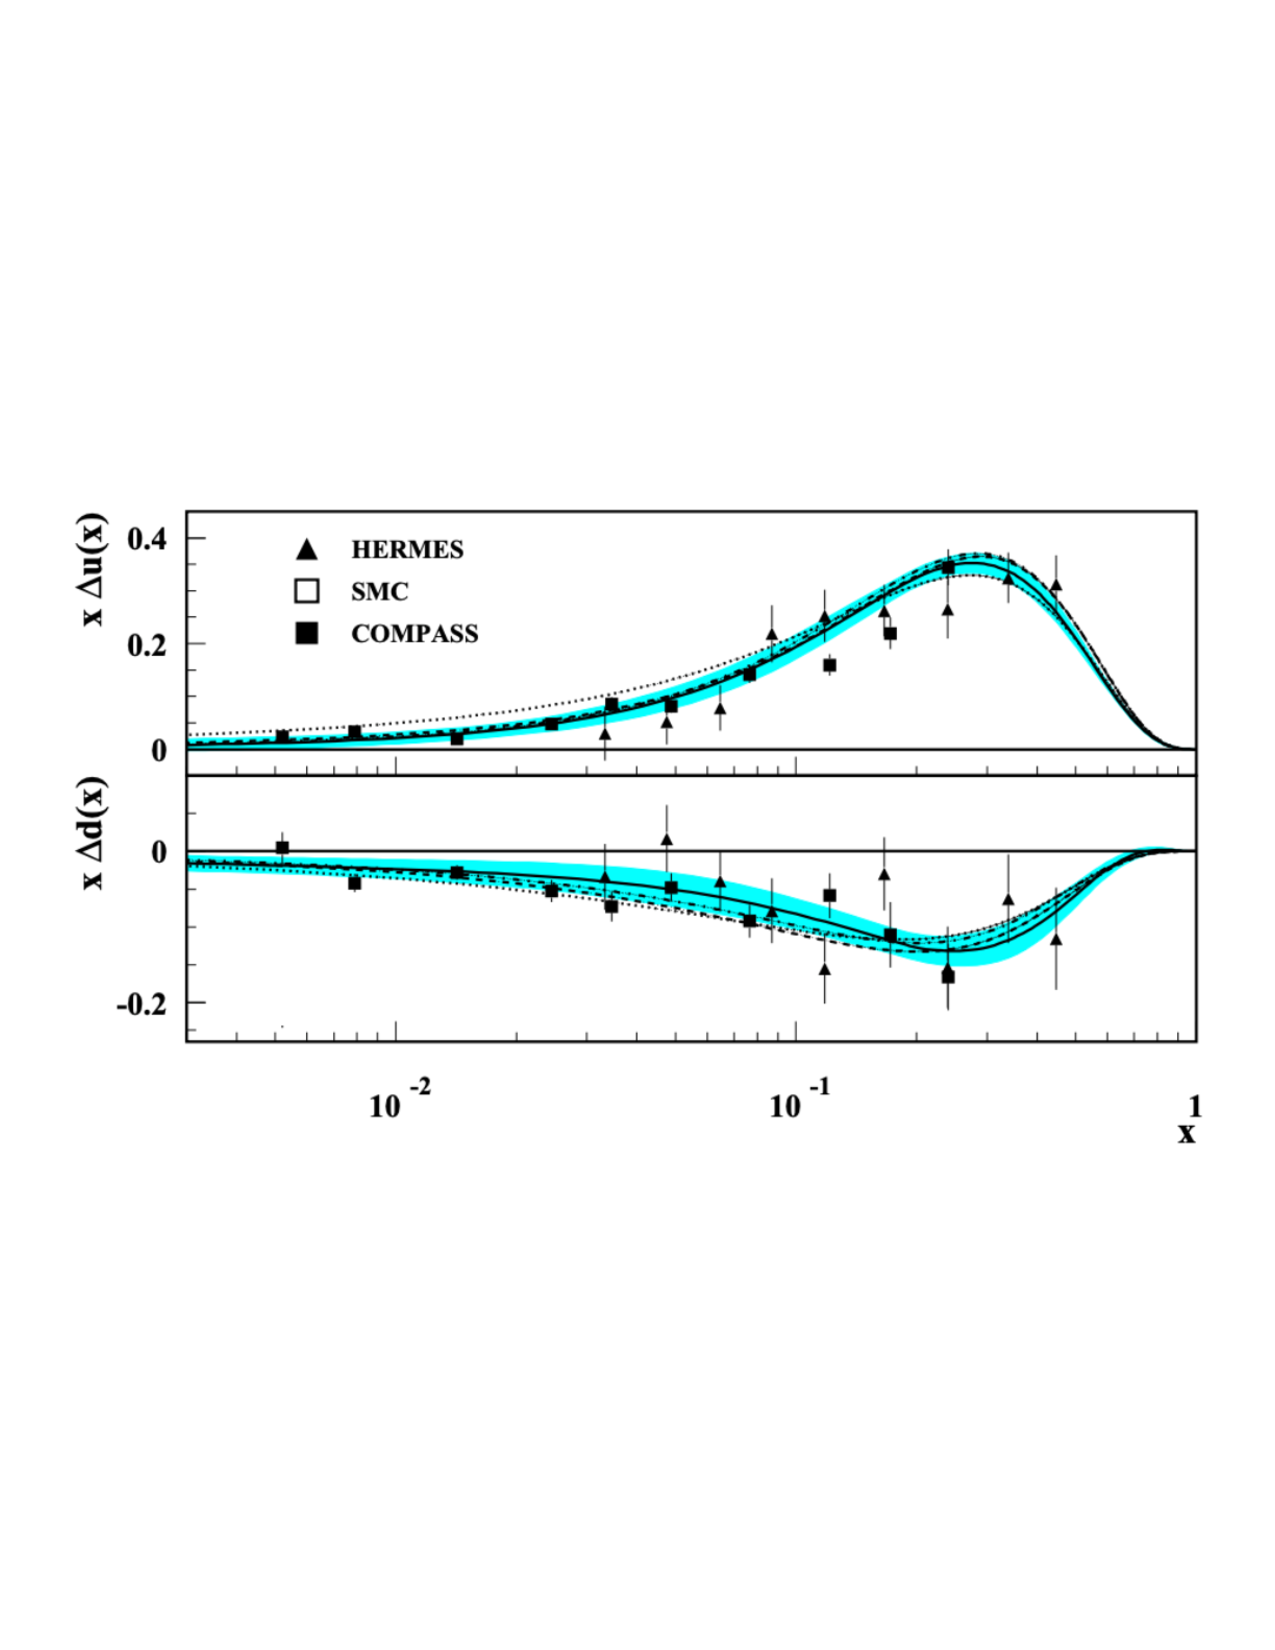
\includegraphics[width=0.5\textwidth,trim=1cm 8cm 1cm 8cm,
    clip]{Proton_g1L}
  \caption{The longitudinally polarized parton distribution functions times the
    momentum fraction for the u-quark (top) and the d-quark (bottom).  Image
    taken from~\cite{Tanabashi:2018oca}}
  \label{fig::Proton_g1L}
\end{figure}

In the parton model the structure function $F_1$ and $F_2$ are related to each
other and to the unpolarized quark number as
\begin{equation}
  F_2(x) = 2xF_1(x) = \sum_q e_q^2x\Big(f^q_1 + f^{\bar{q}}_1 \Big)
\end{equation}
which is known as the Callan-Gross relation~\cite{PhysRevLett.22.156}.  As well
the structure function $g_1$ is related to the helicity distribution, $g_{1L}$,
as
\begin{equation}
  g_1(x) = \frac{1}{2} \sum_q e^2_q g_{1L}(x).
\end{equation}


\section{Transverse Momentum Dependence}
The transverse momentum of the partons is integrated over when measuring the DIS
process.  This is because only the scattered lepton is measured and any
transverse parton motion cannot be measured.  The Drell-Yan
process~\ref{sec::DY} and the SIDIS process~\ref{sec::SIDIS} however are
sensitive to the internal transverse momentum of the partons.  When including
the transverse parton momentum, the most generic leading order quark-quark
correlator can be written~\cite{Mulders:1995dh,Boer:1997nt,Bacchetta:2006tn}

\begin{dmath}
  \label{equ::GeneralQQcorrelator}
  \Theta = \frac{1}{2}\Big[ f_1(x,k_{\bot})\slashed{P} +
    \frac{1}{M}h_1^{\bot}(x,k_{\bot})\sigma^{\mu\nu}k_{\mu}P_{\nu} +
    g_{1L}(x,k_{\bot})\lambda\gamma_5\slashed{P} +
    \frac{1}{M}g_{1T}(x,k_{\bot})\gamma_5\slashed{P}(k_{\bot} \cdot S_{\bot}) +
    \frac{1}{M}h_{1L}(x,k_{\bot})\lambda
    i\sigma_{\mu\nu}\gamma_5P^{\mu}k_{\bot}^{\nu} +
    h_1(x,k_{\bot})i\sigma_{\mu\nu}\gamma_5P^{\mu}S_{\bot}^{\nu} +
    \frac{1}{M^2}h_{1T}^{\bot}(x,k_{\bot})i\sigma_{\mu\nu}\gamma_5P^{\mu} \Big(
    k_{\bot} \cdot S_{\bot}k_{\bot}^{\nu} - \frac{1}{2}k_{\bot}^2S_{\bot}^{\nu}
    \Big ) +
    \frac{1}{M}f_{1T}^{\bot}(x,k_{\bot})\epsilon^{\mu\nu\rho\sigma}\gamma_{\mu}P_{\nu}k_{\rho}S_{\sigma}
    \Big],
\end{dmath}
\noindent
where $k_{\bot}$ denotes the transverse parton momentum and $S_{\bot}$ denotes
the transverse hadron spin.  Eq.~\ref{equ::GeneralQQcorrelator} includes eight
transverse momentum dependent (TMD) PDFs which are functions of $x$ and
$k_{\bot}$.  The notation used to depict the TMDs functions is the so-called
Amsterdam notation.  The letters represent the different quark polarizations
where $f, g, h$ stand for unpolarized, longitudinally polarized and transversely
polarized respectively.  The subscript 1 denotes leading order and the
subscripts $T$ and $L$ denote a transversely polarized hadron and a
longitudinally polarized hadron respectively.  Finally the superscript $\bot$
denotes that the distribution is an odd function of $k_{\bot}$ and therefore is
zero when integrated over the parton transverse momentum.  Fig.~\ref{fig::TMDs}
organizes the TMDs by nucleon and quark polarizations and gives a visual of each
TMD's interpretation.

\begin{figure}[h!t]
  \centering
  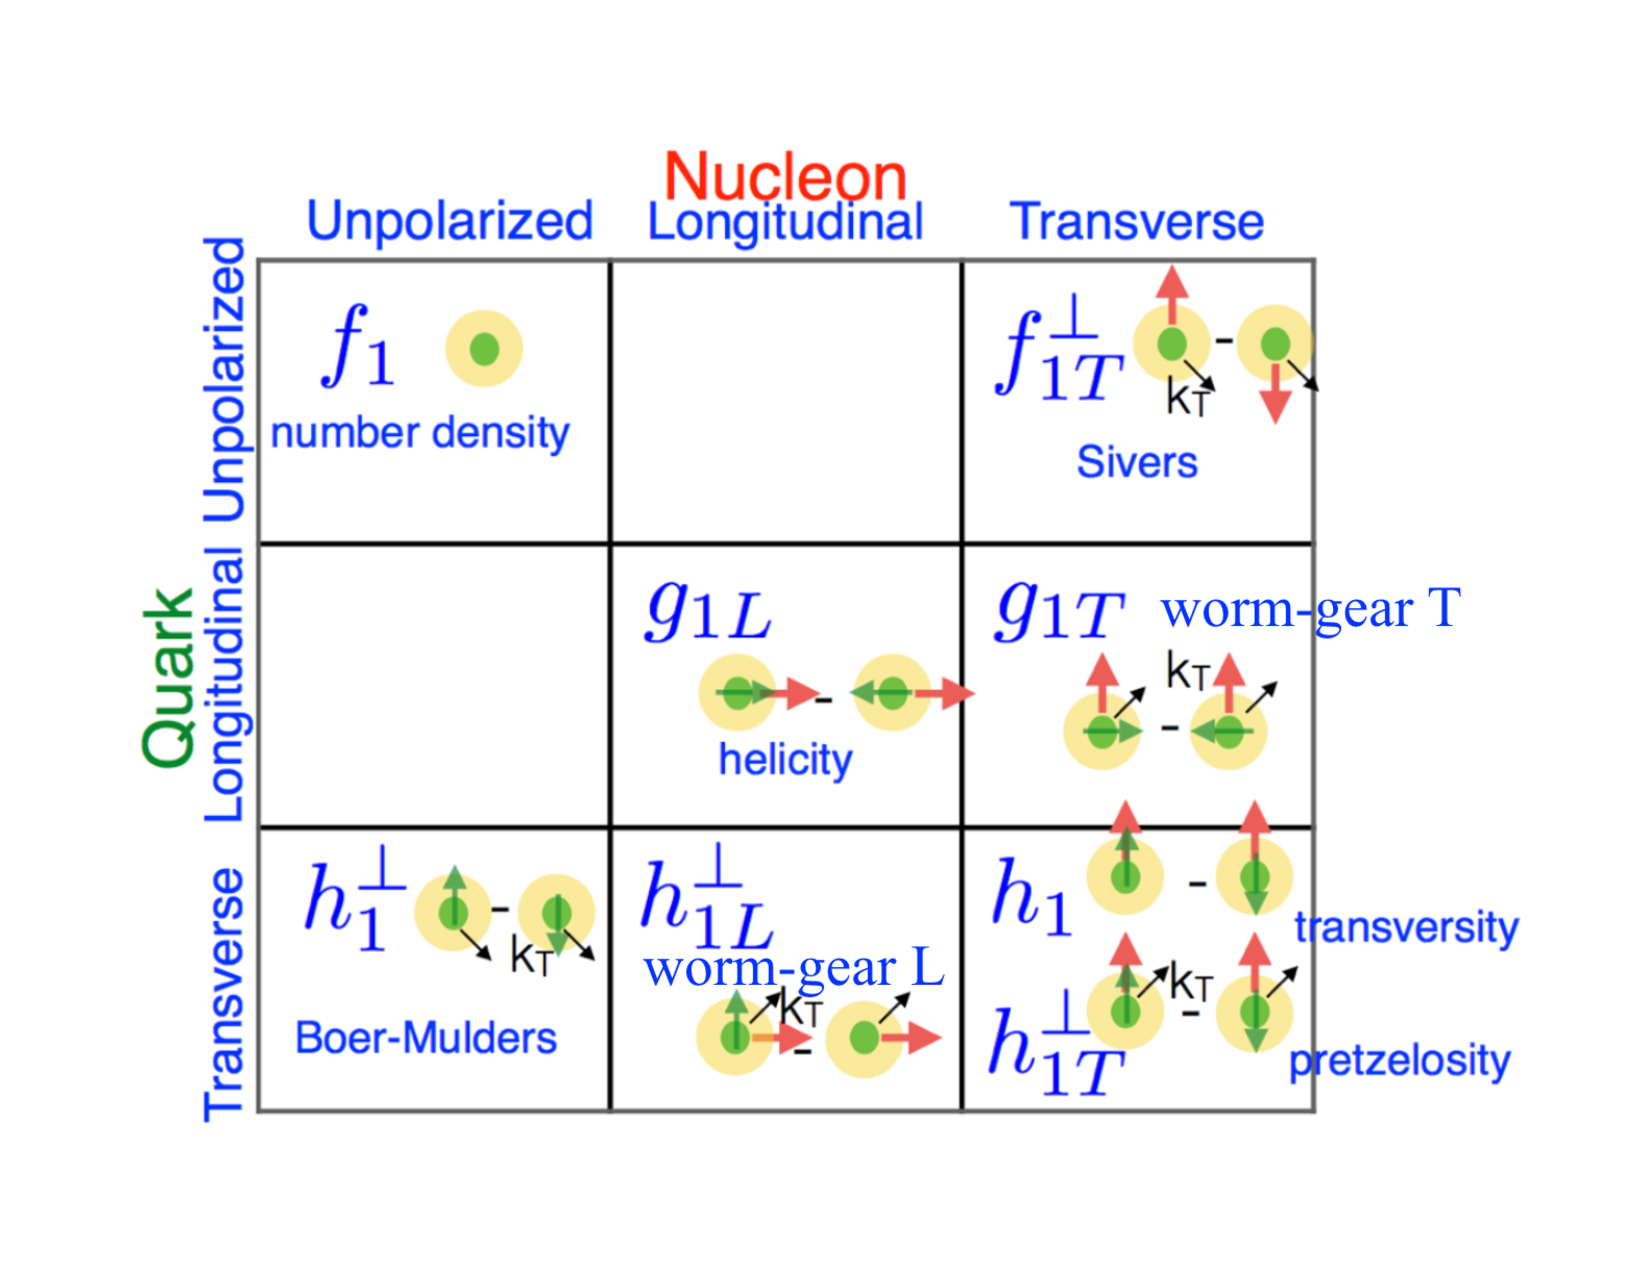
\includegraphics[width=0.6\textwidth, trim=2cm 2cm 2cm 2cm,clip]{TMDs}
  \caption{The eight TMDs needed to describe a spin 1/2 nucleon at leading
    order.  The columns represent the different nucleon polarization and the
    rows represent the different quark polarizations.  The individual figures
    give a visual of the TMD's interpretation.}
  \label{fig::TMDs}
\end{figure}

\subsection{Sivers Distribution}
The Sivers TMD was first purposed to explain large nucleon spin-dependent
asymmetries~\cite{Sivers}.  The interpretation of the Sivers TMD, {\siv}, is
that it gives a correlation between transverse spin of the parent hadron and
transverse momentum of parton.  When viewing the hadron in the direction of it's
momentum, if {\siv} is positive then it is expected that there are more partons
with momentum going left than going right.  Intuitively a non-zero {\siv} would
then imply that the bound quarks carry orbital angular momentum.  As of yet
however, there is no theoretical link between orbital angular momentum and the
Sivers function.

The Sivers function is odd under time reversal.  As a result of this it was
originally believe to be a forbidden correlation.  However it was shown that the
Sivers function could be non-zero from gluon exchange during the initial state
in the Drell-Yan process and during the final state in
SIDIS~\cite{Brodsky:2002cx,Brodsky:2002rv}.  Surprising it was shown that a
non-zeron Sivers function is expected to have opposite sign in SIDIS and
Drell-Yan~\cite{collins_2002}.  That is

\begin{equation}
  f_{1T}^{\bot} |_{Drell-Yan} = - f_{1T}^{\bot} |_{SIDIS}.
\end{equation}

give sivers SIDIS results from HERMES/COMPASS.  Give interpretation

\section{Drell-Yan} \label{sec::DY}

\section{Semi-Inclusive Deep Inelastic Scattering} \label{sec::SIDIS}

\begin{dmath}
  W_{\mu\nu} =
  \Big( \frac{q_{\mu}q_{\nu}}{q^2}-g_{\mu\nu} \Big) \frac{F_1(x, Q^2)}{M} +
  \Big(P_{\mu} - \frac{P \cdot q}{q^2}q_{\mu} \Big)
  \Big(P_{\nu} - \frac{P \cdot q}{q^2}q_{\nu} \Big) \frac{F_2(x, Q^2)}{M^2\nu} +
  i\epsilon_{\mu\nu\rho\sigma}\frac{q^{\rho}}{P \cdot q}
  \Big\{ S^{\sigma}g_1(x, Q^2) +
  \Big( S^{\sigma} - \frac{S\cdot q}{P\cdot q}P^{\sigma}\Big)g_2(x,Q^2) \Big\},
\end{dmath}
\noindent
where $F_1$, $F_2$, $g_1$ and $g_2$ are structure functions which are determined
from experiments.

